% Paths relative to the R10 fragment; requires graphicx.
\begin{figure}[ht]
 \centering
 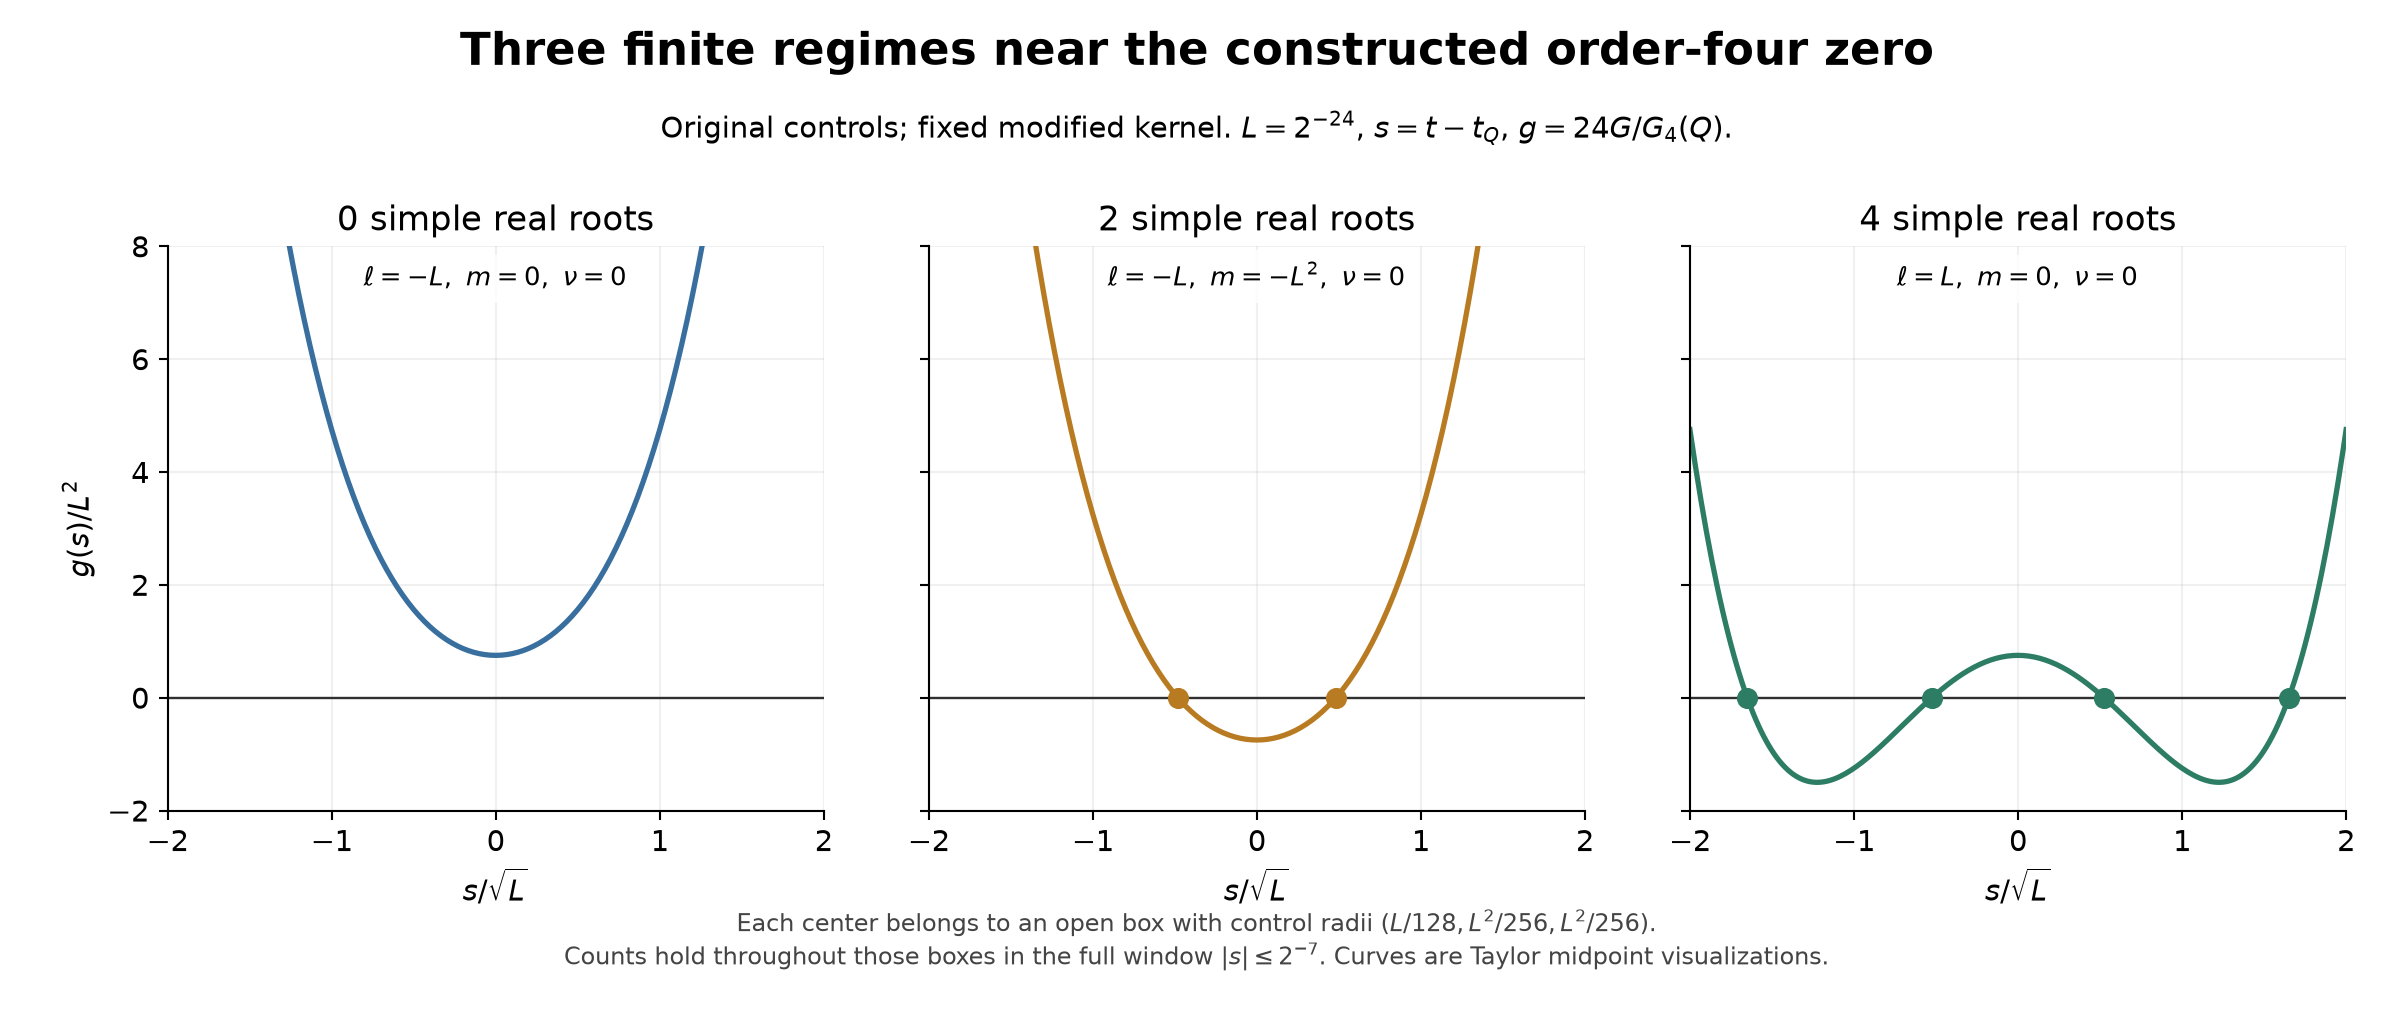
\includegraphics[width=\textwidth]{figures/finite_root_regimes.png}
 \caption{Three root regimes near the constructed order-four zero,
 using $g=24G/G_4(Q)$ and $L=2^{-24}$. The displayed original control
 offsets are centers of open boxes with radii
 $(L/128,L^2/256,L^2/256)$. Every control in those boxes has the
 respective $0$, $2$ or $4$ simple real zeros in the full certified
 window $|s|\leq2^{-7}$. Curves use midpoint Taylor evaluations;
 the nonzero root markers have separate contraction certificates.
 The displayed horizontal range is smaller than the full window.
 A fixed nonzero normalization changes no zeros or multiplicities.}
\end{figure}

\begin{figure}[ht]
 \centering
 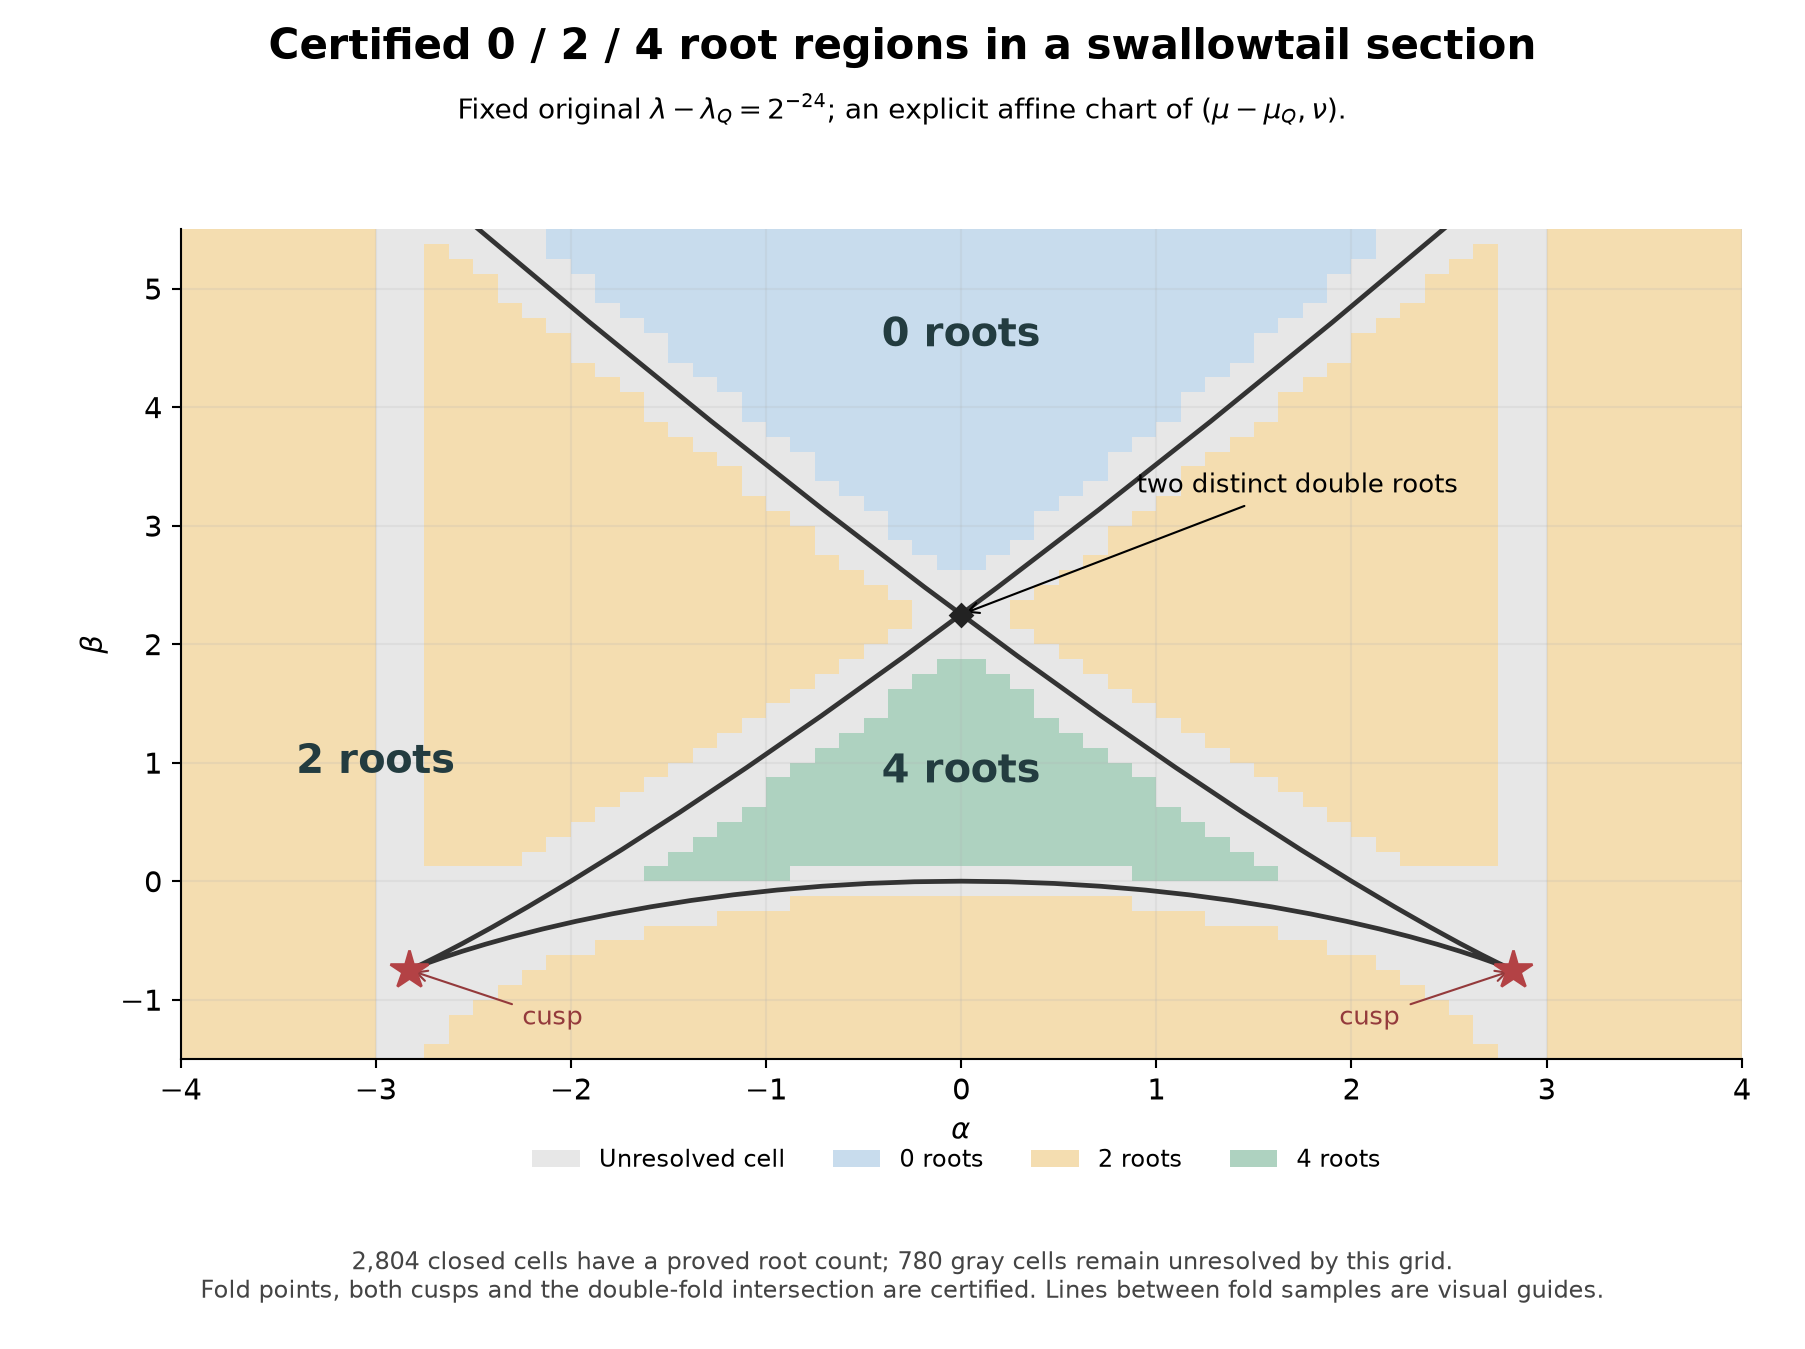
\includegraphics[width=\textwidth]{figures/certified_swallowtail_section.png}
 \caption{A finite section at the original control offset
 $\ell=2^{-24}$. The axes form the explicitly specified affine chart
 of $(m,\nu)$, not an unknown normal-form coordinate transformation.
 Each colored closed cell has a rigorously proved number of simple
 real roots in the common $s$ window: $430$ zero-root cells, $2184$
 two-root cells and $190$ four-root cells. The $780$ gray cells are
 unclassified by this grid certificate; they are not assumed to
 consist of multiple roots. Both cusps and the simultaneous pair
 of distinct double zeros are separately certified. Black lines
 connect $81$ certified fold points as visual guides. Uniform
 surface and cusp graph theorems establish the underlying continuum
 geometry independently of these line segments.}
\end{figure}
